%%%%%%%%%%%%%%%%%%%%%%%%%%%%%%%%%%%%%%%%%%%%%%%%%%%%%%%%%%%%%%%%%%%%%%%
%%%%%%%%%%%%%%%%%%%%%%%%%%%%%%%%%%%%%%%%%%%%%%%%%%%%%%%%%%%%%%%%%%%%%%%
%%%%%                                                                 %
%%%%%     <file_name>.tex                                             %
%%%%%                                                                 %
%%%%% Author:      <author>                                           %
%%%%% Created:     <date>                                             %
%%%%% Description: <description>                                      %
%%%%%                                                                 %
%%%%%%%%%%%%%%%%%%%%%%%%%%%%%%%%%%%%%%%%%%%%%%%%%%%%%%%%%%%%%%%%%%%%%%%
%%%%%%%%%%%%%%%%%%%%%%%%%%%%%%%%%%%%%%%%%%%%%%%%%%%%%%%%%%%%%%%%%%%%%%%

\chapter{Schematics}
\label{ch:schemata}
This appendix contains all detailled schemata of this thesis. \\
TODO: some illustrations about color and naming conventions!

\minilof

\begin{landscape}
\begin{figure}[t!]

\centering
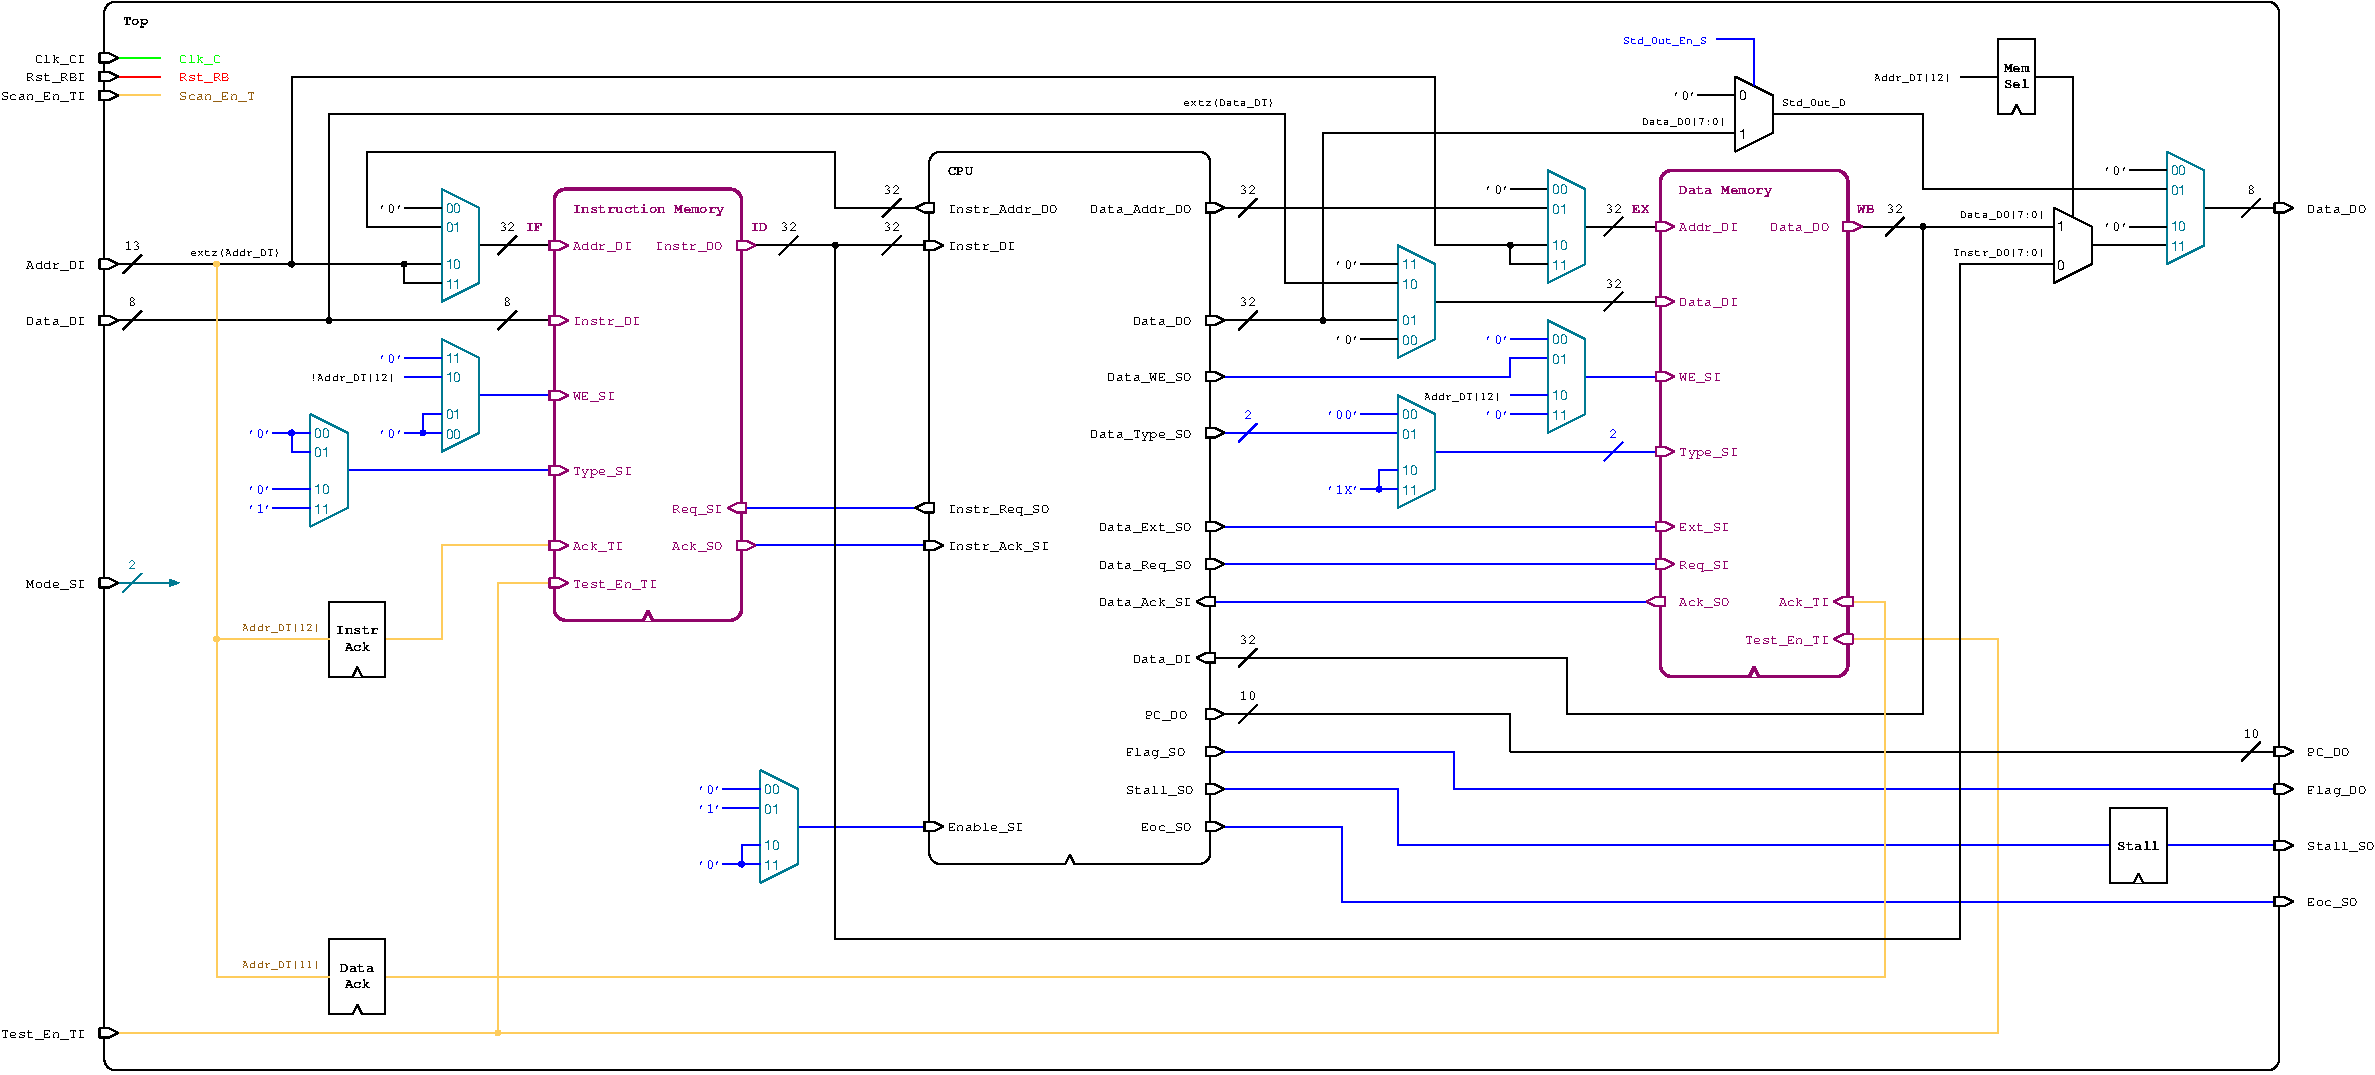
\includegraphics[scale=0.8]{figures/top.pdf}
\caption{Main schema of the top level design}
\label{fig:top_schema}
\end{figure}
\end{landscape}
\cleardoublepage
%% CPU %%
\begin{landscape}
\begin{figure}[t!]

\centering
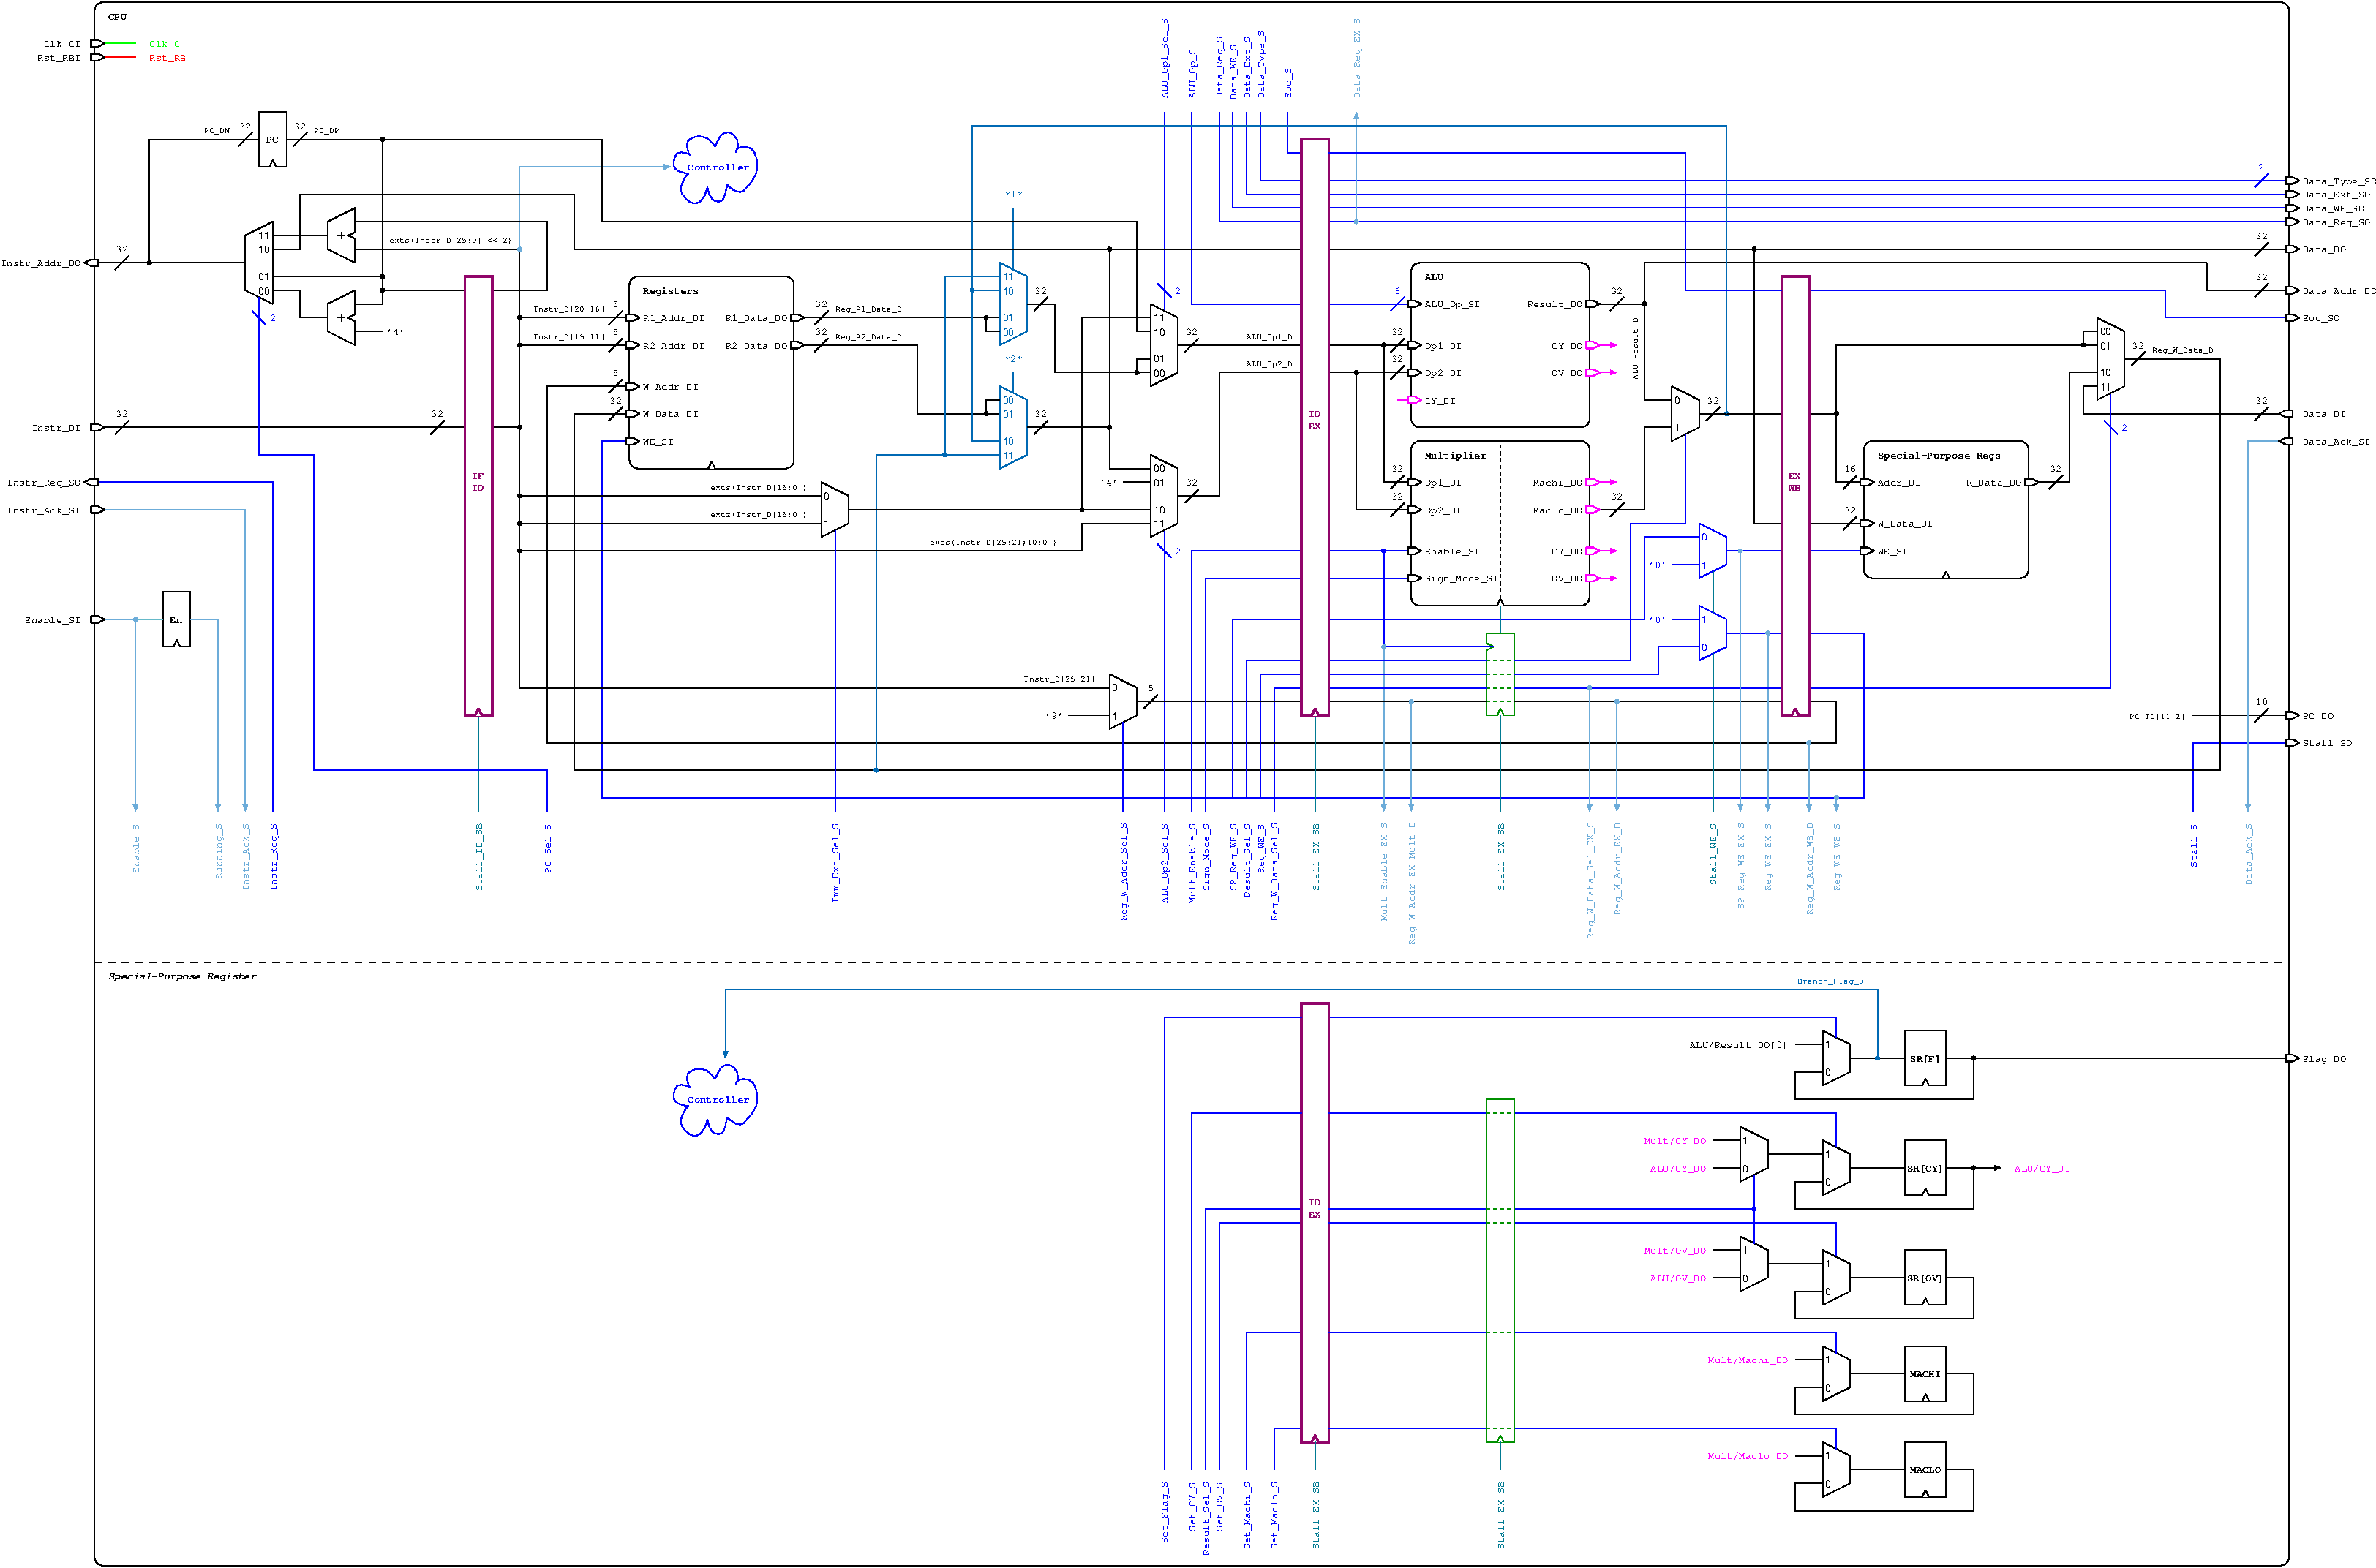
\includegraphics[scale=0.35]{figures/cpu.pdf}
\caption{Main schema of the CPU}
\label{fig:cpu_schema}
\end{figure}
\end{landscape}

\cleardoublepage
%% ALU %%
\begin{figure}[t!]

\centering
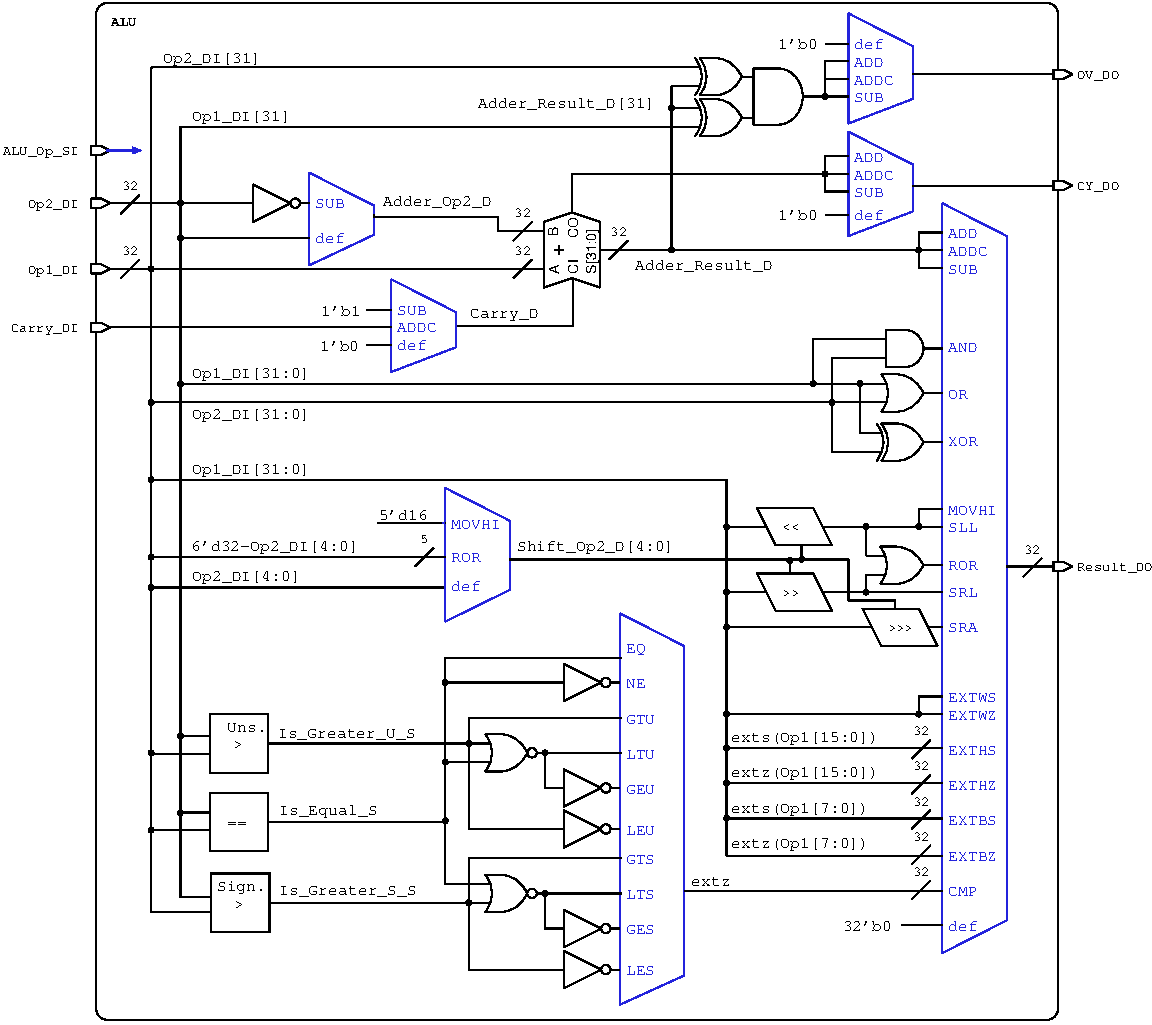
\includegraphics[scale=0.9]{figures/alu_schema.pdf}
\caption{Main schema of the ALU}
\label{fig:alu_schema}
\end{figure}
\clearpage

\begin{landscape}

\begin{figure}[t!]

%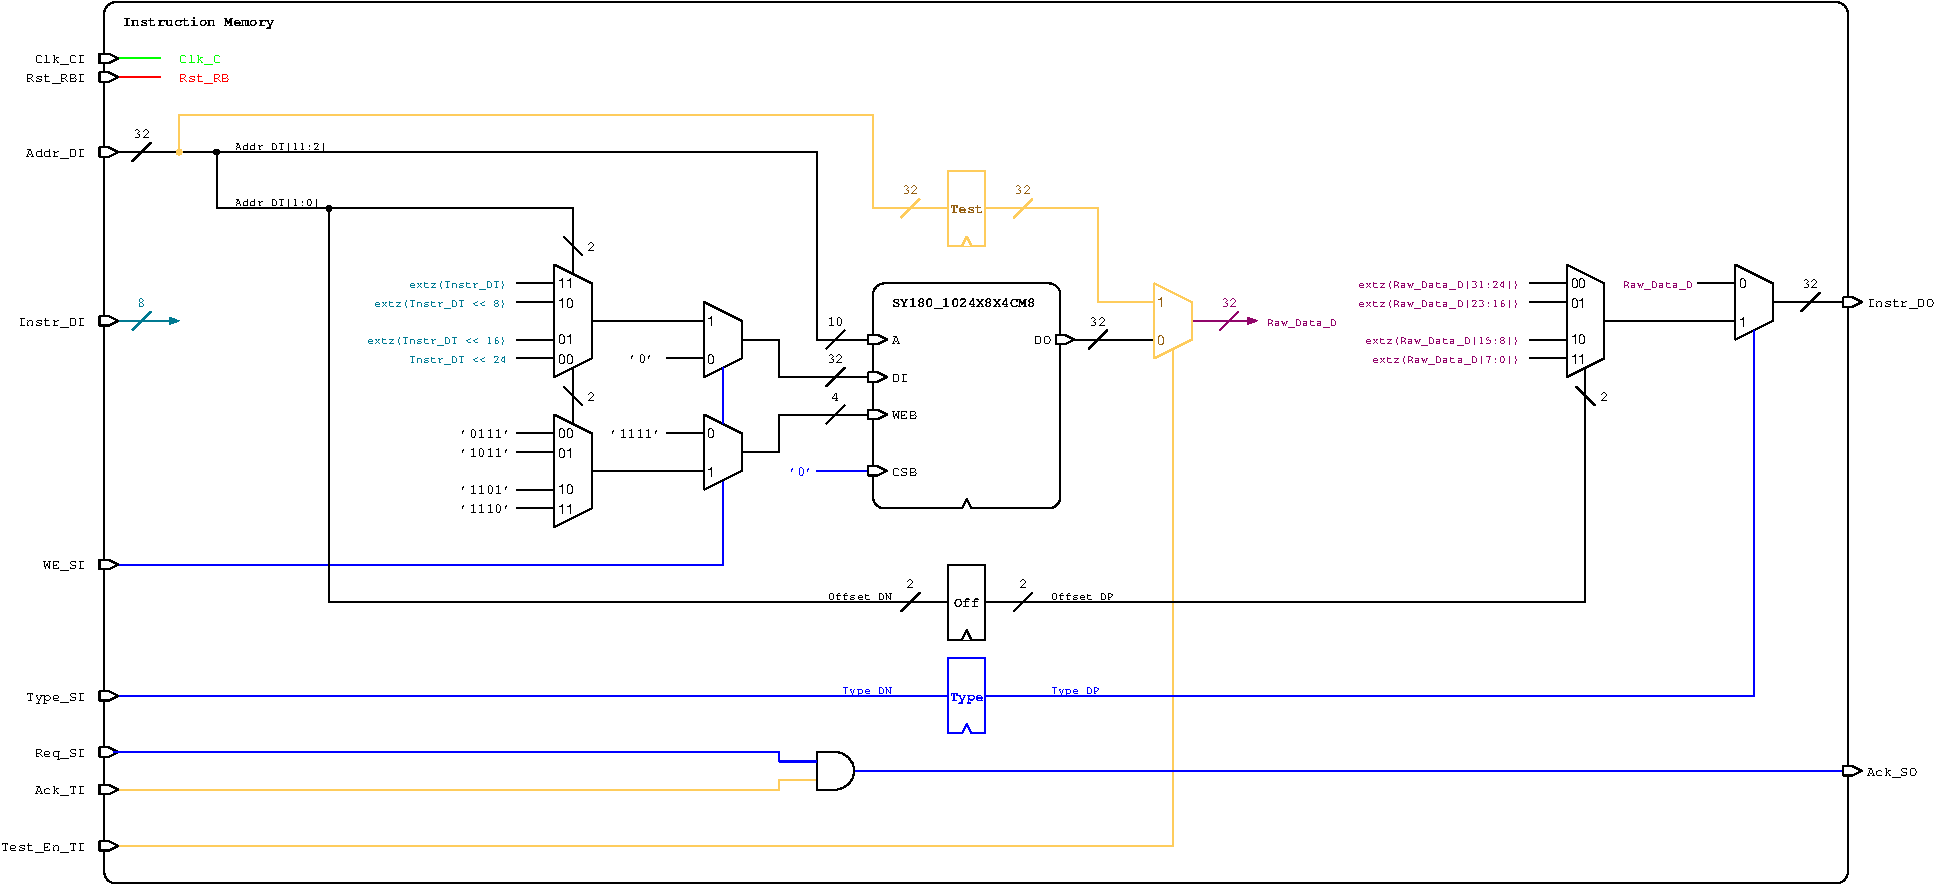
\includepdf{figures/instr_mem.pdf}
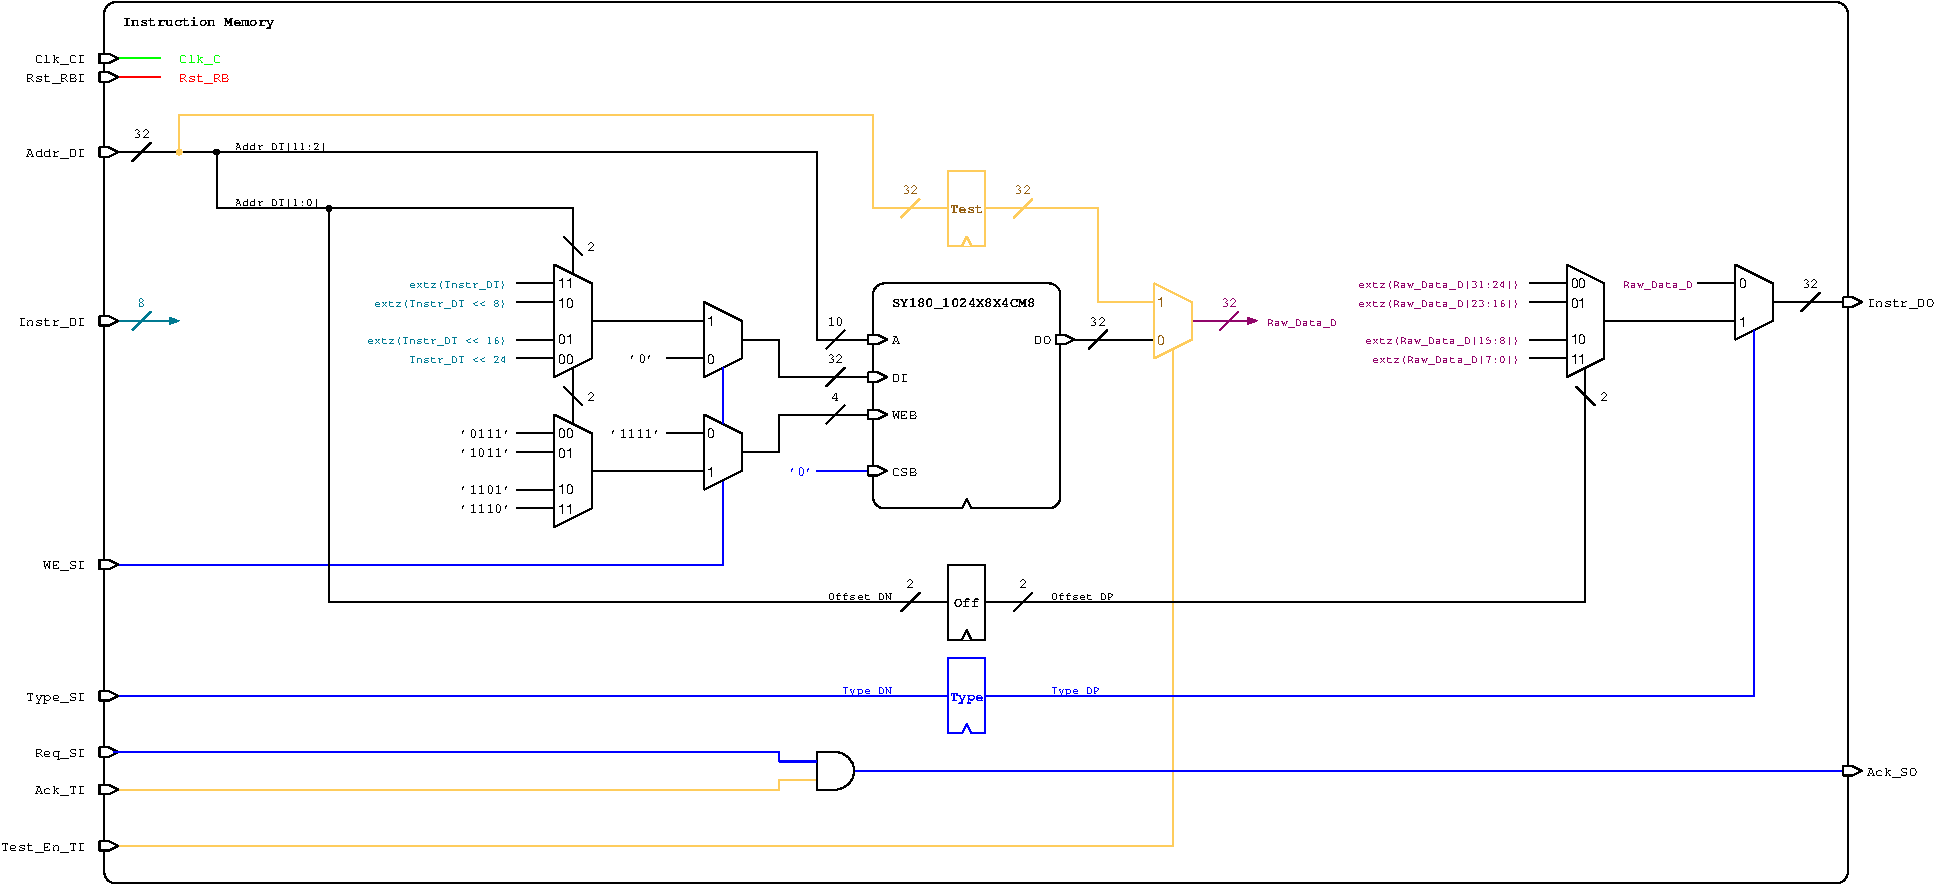
\includegraphics[scale=0.65]{figures/instr_mem.pdf}
\caption{Main schema of the instruction memory}
\label{fig:instr_mem}

\end{figure}
\end{landscape}
\clearpage
%\begin{figure}[t!]
\addtocounter{figure}{1}

\addcontentsline{lof}{section}{\Alph{chapter}.\arabic{figure}.\hspace{0pt} Main schema of the data memory}
\mtcaddchapter
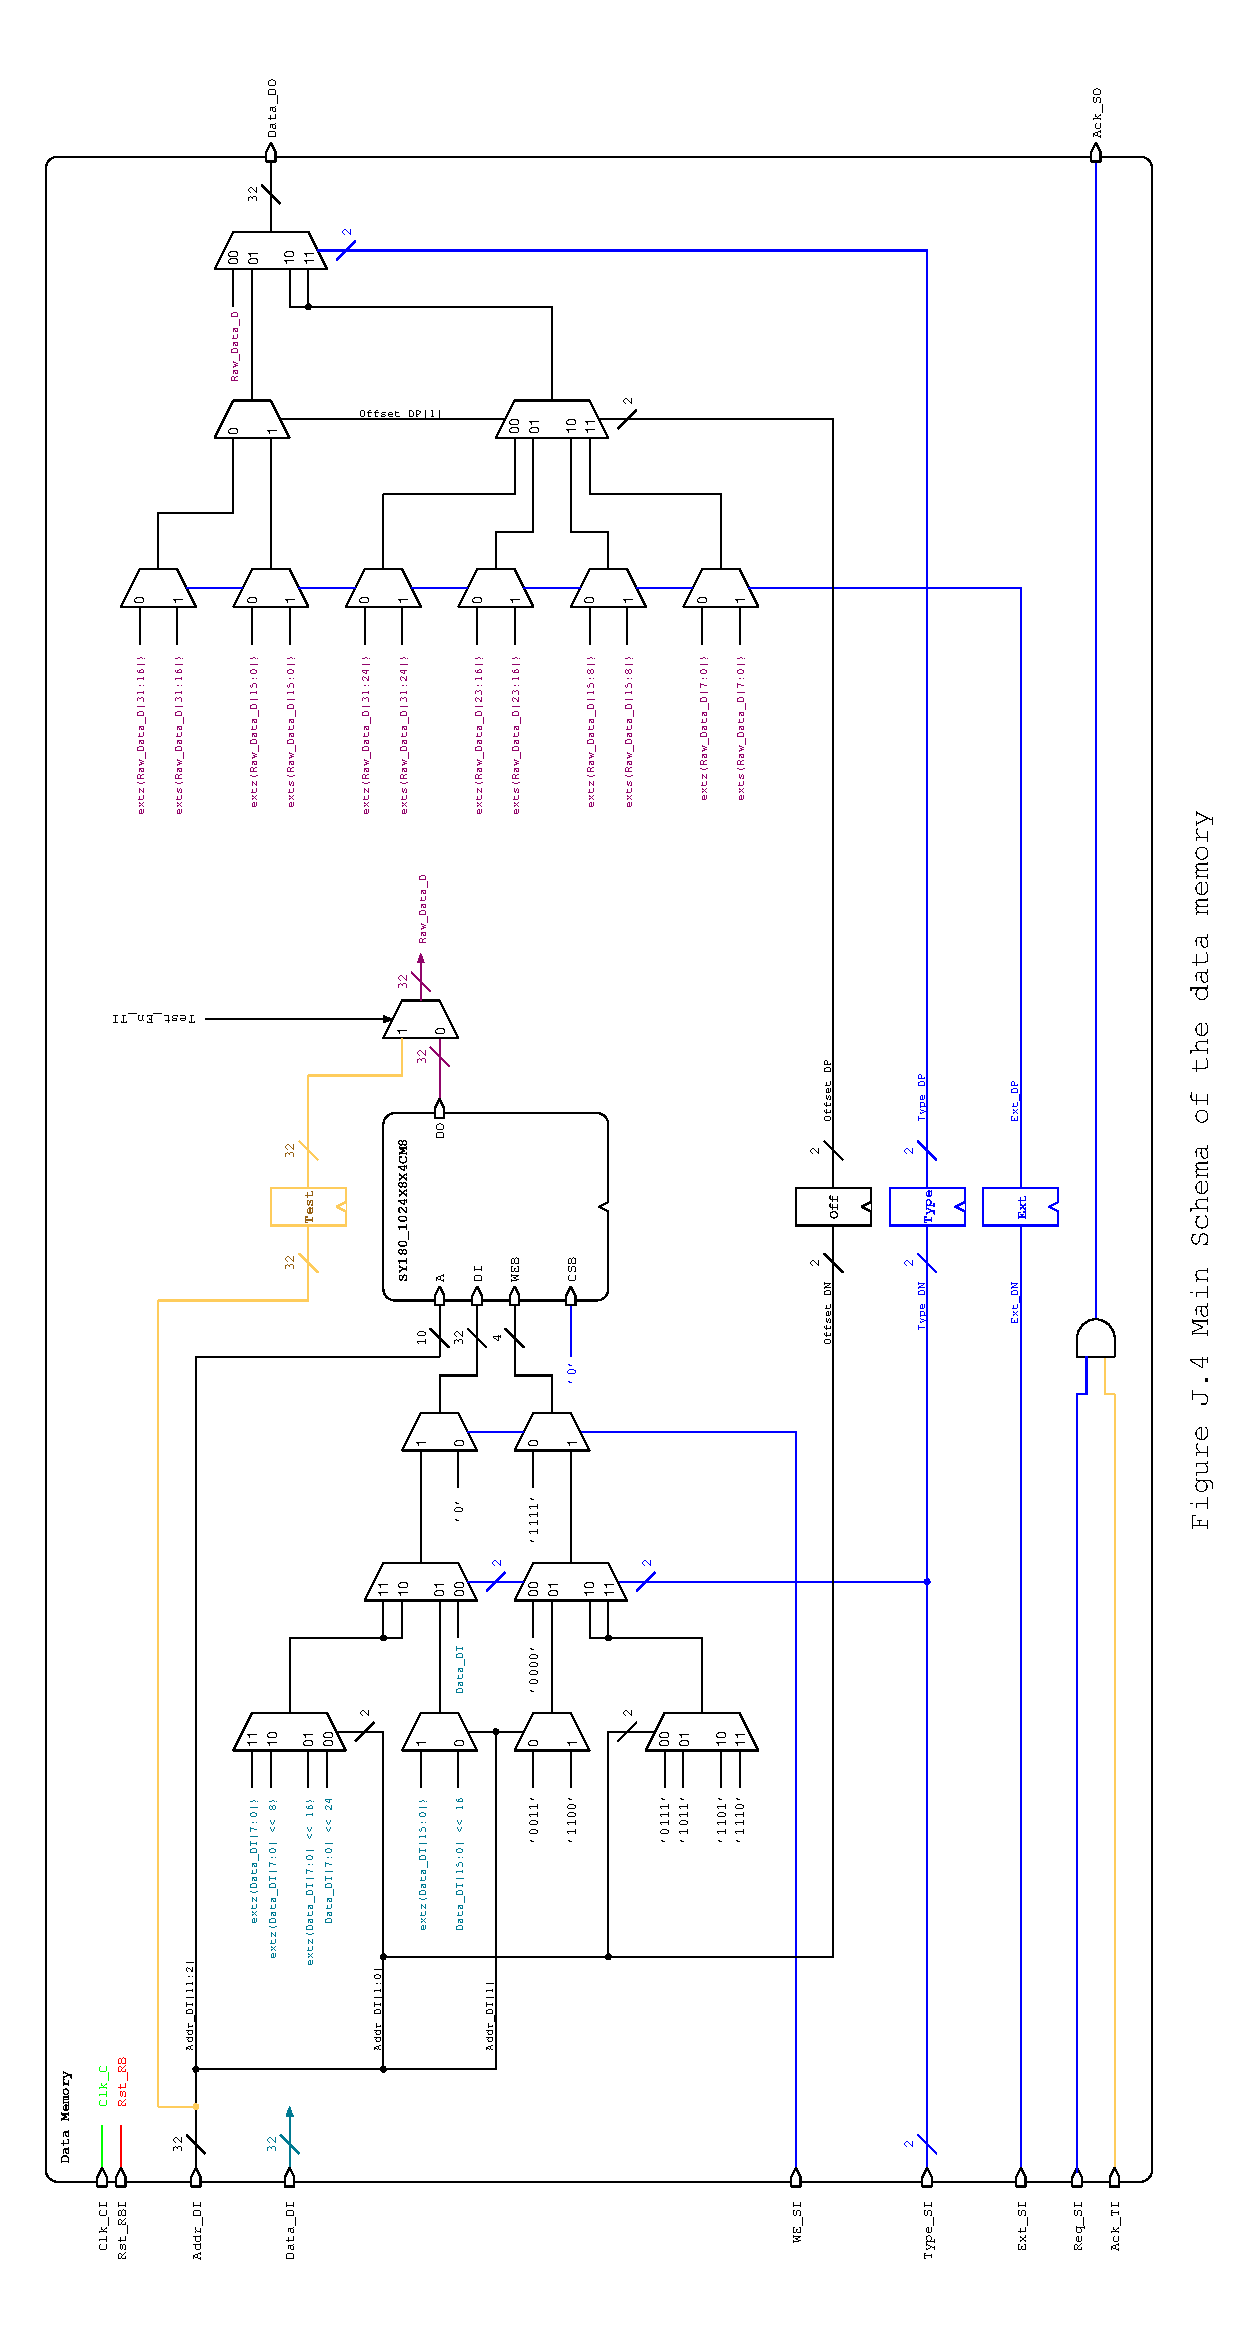
\includepdf{figures/data_mem.pdf}
%\caption{Schema of the data memory}

%\end{figure}

\cleardoublepage

